\clearpage
%//==============================--@--==============================//%
%\vspace{-1em}
\subsection{P4 | Simulação do sistema completo}
\label{subsec:P4}
%//==============================--A--==============================//%
\vspace{-0.5em}
\subsubsection{a) Gráficos das variáveis relevantes}
\label{subsubsec:P4a}

%%% 
\vspace{-1em}
\noindent\begin{minipage}[t]{0.45\textwidth}
\begin{lstlisting}[title=Pergunta 4, frame=tlrb]{P4-a}
%% Function calls

% init concentration
c = concentration(); % same function as in P1

% init effect
u = Hill(c);
% init volume growth
v = Tumor(u);
% plot
PlotRelevantVariables(c, d, v, u);
%%
function v = Tumor(u)
    %tumor growth variables 
    a = 0.09; b = 1; Kt=10; h = 1; p0 = 1; %1mm^3 
    size = length(u);
\end{lstlisting}
\end{minipage}
\hfill \noindent\begin{minipage}[t]{0.45\textwidth}
\begin{lstlisting}[title = (continuação), frame=tlrb]{P4-a}
    %create logistic equation
    l = @(v,u)a*v*(1-v./Kt) - b*u.*v;
    %preallocating for speed
    v = zeros(1,size); v(1) = p0; %<- v0
    %simple Euler's integration
    for i = 1:(size - 1)
        v(i+1) = v(i) + h*l(v(i),u(i));
    end
end
%%
function u = Hill(c)
    %half maximal effect
    c50 = 7.1903;
    %create Hill's equation: Pharmacodynamic model
    u = c(2,:)./(c50 + c(2,:));
end
\end{lstlisting}
\end{minipage}

\vspace{1em}
 \hspace*{-1.98cm}\begin{tabular}{C{9cm}  L{8 cm}}
        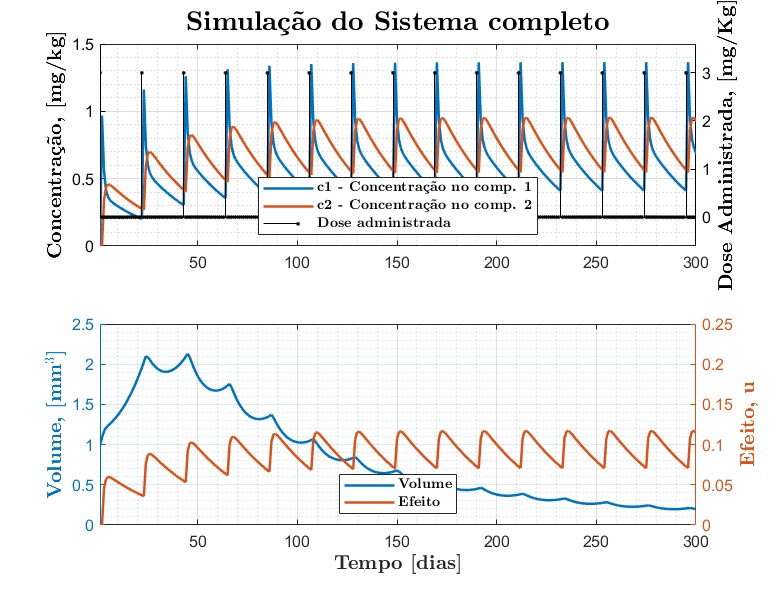
\includegraphics[width=\linewidth]{img/perguntas/P4/P4-a.png} & 
        \vspace{-2.5em} \captionof{figure}{\textbf{Simulação do sistema completo}.} 
        \vspace{0.5em}
        \hspace*{1em} Procedeu-se à simulação do sistema completo, considerando uma administração equiespaçada de período $T = 21$d (utilizada em alíneas anteriores) mediante uma janela temporal de 300 dias. O tumor, após atingir 200\% do volume inicial, é lentamente erra- dicado, aparente na diminuição de volume com a constante administração do fármaco.
        
        \hspace*{1em} A característica ondulatória da evolução do volume do tumor deve-se à presença reduzida do fármaco no organismo, conse- quência da dosagem de $3$ mg/kg.
    \end{tabular}
%//==============================--B--==============================//%
\subsubsection{b) Otimização do espaçamento entre aplicações do fármaco}
\label{subsubsec:P4b}
%%% BEGIN TABULAR
\vspace{-1em}
\begin{tabular}{c c}%%
    \hspace*{-1em}\noindent\begin{minipage}[t]{0.475\textwidth}
\begin{lstlisting}[title=Pergunta 4 - Aquisição do espaçamento,frame=tlrb]{P4-b}
function T = Optimal()
    %declare requerimen
    opVolume = 0.10; N = 25; d = zeros(1,N) + 3;
    
    for T = 1:21
        clear dosage; dosage = upsample(d,T); 

        % Calculate volume evolution
        c = concentration(dosage);
        u = Hill(c);
        v = Tumor(u);

        % evaluate volume at 25 day mark
        if v(25) >= opVolume
            break
        end
    
    end
    fprintf("Optimal periodicity: \%i days\textbackslash n", T);
    
end
\end{lstlisting}
    \end{minipage} &\
    \noindent\begin{minipage}[t]{0.5\textwidth}
        \begin{figure}[H]
            \vspace{-0.4em}
            \hspace*{-1.25em}
            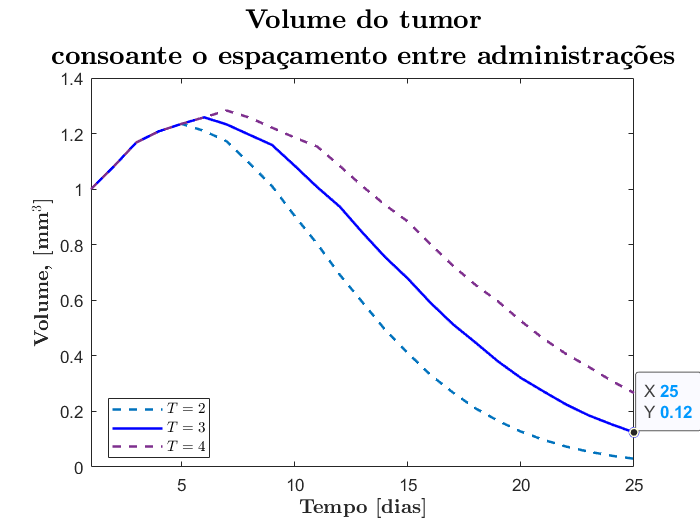
\includegraphics[width = 1\linewidth]{img/perguntas/P4/P4-b.png}
            \caption{Evolução do volume do tumor consoante 3 espaçamentos adjacentes. A \textcolor{blue}{azul} verifica-se a curva com o valor ótimo para solucionar os requerimentos.}
            \label{fig:P4-b}
        \end{figure}
    \end{minipage}
\end{tabular}
%%% END TABULAR

%//==============================--@--==============================//%
